%%%%%%%%%%%%%%%%%%%%%%%%%%%%%%%%%%%%%%%
%                                     %
%    Header Start                     %
%                                     %
%%%%%%%%%%%%%%%%%%%%%%%%%%%%%%%%%%%%%%%

% Din A 4 page with font size 12
%\documentclass[a4paper, twosides, 12pt]{article}
\documentclass[12pt,a4paper]{article}
\usepackage[english]{babel}
\usepackage[T1]{fontenc}
\usepackage[utf8]{inputenc}

%von niko
%\usepackage[margin=1.5in]{geometry}
%\usepackage{algorithmic}
%\usepackage{subcaption}
%\usepackage{lettrine}
%\usepackage[sc,osf]{mathpazo}
%\usepackage{booktabs}
% Es wird nicht eingerckt
\parindent=0mm

% arabic numbers for page numbering
\pagenumbering{roman}

% Definition der Ränder
\usepackage[paper=a4paper,left=30mm,right=30mm,top=25mm,bottom=25mm]{geometry}

% for declaring and using colors
\usepackage[table]{xcolor}
% define color values here
\definecolor{myblue}{rgb}{0.94, 0.97, 1.0}
\definecolor{Gray}{gray}{0.8}

% for apacite references
% \usepackage{apacite}
% \bibliographystyle{apacite}

% add references to Table of Contents
\usepackage[nottoc]{tocbibind}


% environment for definitions
\newtheorem{definition}{Definition}

\newtheorem{problem}[definition]{Problem}

% enumerate change
\usepackage{paralist}

% for romanic numbers
\newcommand{\RM}[1]{\MakeUppercase{\romannumeral #1{}}}

% for inserting graphics
\usepackage{graphicx}
\usepackage{subfigure}
\usepackage{tikz}
\usetikzlibrary{arrows,shapes,positioning,shadows,trees}
\tikzset{
  basic/.style  = {draw, text width=3cm, drop shadow, font=\sffamily, rectangle},
  root/.style   = {basic, rounded corners=2pt, thin, align=center,
                   fill=green!30},
  level 2/.style = {basic, rounded corners=6pt, thin,align=center, fill=green!60,
                   text width=8em},                                                  
  level 3/.style = {basic, thin, align=left, fill=blue!60, text width=6.9em}
}
\usepackage{wrapfig}

%\usepackage{pstricks}

% for inserting tables
\usepackage{tabularx, multirow, array, dcolumn}

% for mathematical symbols
\usepackage{amsmath}
\usepackage{amssymb}
\usepackage{latexsym}

% for graphics
\usepackage{tikz}
\usetikzlibrary{arrows,positioning}
\usepackage{color}

%for ipa
\usepackage{tipa}

% pdf LaTeX for linguistic examples
\usepackage{linguex}

%%for OT tables
\usepackage{pifont}    %for pointing hand
\usepackage{arydshln}    %for dashed lines
\usepackage{rotating}    %for angled text

% for inserting pdfs
\usepackage{pdfpages} 

% for inserting trees
\usepackage{qtree}
%\usepackage{ps-trees}

% for line distance
\usepackage{setspace}

% for thick lines
\usepackage{booktabs}

% for footer and header
\usepackage{fancyhdr}

%resizing
\usepackage{adjustbox}

% landscape format
\usepackage{lscape}
% for caption formatting
\usepackage{caption}

% for quotation marks
\newcommand{\Gu}{\glqq{}}		% quotation marks top
\newcommand{\Go}{\grqq\xspace} 	% quotation marks bottom
\newcommand{\Ga}{\textquotedblleft{}} % american quotation marks top start
\newcommand{\Ge}{\textquotedblright\xspace} % american quotation marks top end
\newcommand{\Tg}[1]{\textsubscript{#1}}		% lower
\newcommand{\Hg}[1]{\textsuperscript{#1}}	% higher
\newcommand{\leer}{\vspace*{\baselineskip}}% empty line

% reference with \tab, \fig, \sec to tables, graphics, and paragraphs
\usepackage{titleref}
\usepackage{prettyref}
\newrefformat{tab}{siehe Tab. \ref{#1} "\titleref{#1}" auf der Seite \pageref{#1}}% tables
\newrefformat{fig}{siehe Fig. \ref{#1} "\titleref{#1}" auf der Seite \pageref{#1}}% graphics
\newrefformat{sec}{siehe Abschnitt \ref{#1} "\titleref{#1}" auf der Seite \pageref{#1}}% paragraphs
%\pageref{#1}

%changes the numbering of figure and table
\numberwithin{figure}{section}
\numberwithin{table}{section}
\numberwithin{definition}{section}

% heading tweaks
\usepackage{titlesec}
\titleformat{\section}
{\normalfont\Large\bfseries}
{\thesection}
{1em}
{}
\titleformat{\subsection}
{\normalfont\Large\bfseries}
{\thesubsection}
{1em}
{}
\titleformat{\subsubsection}
{\normalfont\Large\bfseries}
{\thesubsubsection}
{1em}
{}

\newcommand{\HRule}{\rule{\linewidth}{0.5mm}}

% global scaling of table size
\usepackage{etoolbox}

\AtBeginEnvironment{tabular}{\scriptsize}
\AtBeginEnvironment{tabularx}{\scriptsize}

% Bibliography
\usepackage[style=authoryear,backend=biber]{biblatex}
\addbibresource{bibliography.bib}

%%%%%%%%%%%%%%%%%%%%%%%%%%%%%
%                           %
%      Document Start       %
%                           %
%%%%%%%%%%%%%%%%%%%%%%%%%%%%%
\begin{document}
\begin{titlepage}
\begin{center}


% Upper part of the page. The '~' is needed because \\
% only works if a paragraph has started.
%\\textsc{includegraphics[width=0.68\textwidth]{bilder/unilogo.png}~\\[1.5cm]
%~\\[1.5cm]
%\vspace{-1.0cm}}

\textsc{\LARGE Master's Thesis}\\[0.8cm]

\textsc{\large in Computational Linguistics}\\[0.5cm]

% Title
\HRule \\[0.4cm]
{  \bfseries \fontsize{22}{37} \selectfont Deconstructing Constructed Languages}\\
\vspace{0.4em}

\HRule \\[1.5cm]



% Author and supervisor
\begin{minipage}{0.4\textwidth}
\begin{flushleft} \large
\emph{Author:}\\
Connor \textsc{Kirberger}
\end{flushleft}
\end{minipage}
\begin{minipage}{0.5\textwidth}
\begin{flushright} \large
%\emph{1st Examiner \& Supervisor:} \\
\emph{Supervisors:} \\
Çağrı \textsc{Çöltekin} \\
Christian \textsc{Bentz}\\
\end{flushright}
\end{minipage}


\vfill



\textsc{\large Seminar f\"ur Sprachwissenschaft\\Eberhard-Karls-Universit\"at T\"ubingen}\\[1.5cm]



% Bottom of the page
{\large December 2023}

\end{center}
\end{titlepage}


%---------------------
% Ende der Titelseite
%---------------------

%----------------------------
% Selbstständigkeitserklrung
%----------------------------

\noindent

Hiermit versichere ich, dass ich die Arbeit selbständig verfasst, keine anderen als die angegebenen Hilfsmittel und Quellen benutzt, alle wörtlich oder sinngemäß aus anderen Werken übernommenen Aussagen als solche gekennzeichnet habe und dass die Arbeit weder vollständig noch in wesentlichen Teilen Gegenstand eines anderen Prüfungsverfahrens gewesen ist und dass die Arbeit weder vollständig noch in wesentlichen Teilen bereits veröffentlicht wurde sowie dass das in Dateiform eingereichte Exemplar mit den eingereichten gebundenen Exemplaren übereinstimmt.\\[4em]
I hereby declare that this paper is the result of my own independent scholarly work.
I have acknowledged all the other authors' ideas and referenced direct quotations
from their work (in the form of books, articles, essays, dissertations, and on the
internet). No material other than that listed has been used.
\\[18mm]
T\"ubingen, \today \hspace{6.0cm} \\%[10mm]\\
\begin{flushright}

\rule{0.4\textwidth}{0.2pt}\\
Firstname Surname
\end{flushright}
\pagestyle{empty}
\newpage

% inserting official anti-plagiarism statement
% \includepdf{antiplagiatserklaerung.pdf}
\newpage
%------------
% Textanfang
%------------

%% Inhaltsverzeichnis
\tableofcontents
\thispagestyle{empty}
%% Anderthalbzeiliger Zeilenabstand ab hier
\onehalfspacing
%\singlespacing

%% Keine Seitenzahl
\pagestyle{empty}

%% Beginn einer neuen Seite
\newpage

%% Abstract
\abstract{

Write the abstract here.
}
\newpage

%% Beginn einer neuen Seite
%\newpage

%%list of figures
\listoffigures
% list of tables
\listoftables


% list of abbreviations
\section*{List of Abbreviations}
\addcontentsline{toc}{section}{List of Abbreviations}

\begin{tabular}{lcl}
\textbf{NLP} & ~~~ & Natural Language Processing \\
\textbf{PCA} & ~~~ & Principle Component Analysis \\
\textbf{TF-IDF} & ~~~ & Term Frequency - Inverse Document Frequency \\
\textbf{RNN} & ~~~ & Recurrent Neural Network \\
\textbf{LSTM} & ~~~ & Long Short-Term Memory \\
\textbf{SVM} & ~~~ & Support Vector Machine \\
\textbf{XML} & ~~~ & eXtensible Markup Language \\
\textbf{TTR} & ~~~ & Type-Token Ratio \\
\textbf{MATTR} & ~~~ & Moving-Average Type-Token Ratio \\
\textbf{IAL} & ~~~ & International Auxiliary Language \\
\textbf{SVO} & ~~~ & Subject-Verb-Object \\

\end{tabular}
\newpage

%\listoftables
%\newpage

%% header with section heading and right-aligned page number
\pagestyle{fancy}
\fancyhf{}
\fancyhead[L]{\textcolor{gray}{\slshape\nouppercase{\rightmark}}}
\fancyhead[R]{\thepage}
\fancyfoot[R]{\textcolor{gray}{Seminar für Sprachwissenschaft Universität Tübingen}}
\renewcommand{\headrulewidth}{0.4pt}

\renewcommand{\headrulewidth}{0.5pt}
\renewcommand{\footrulewidth}{0.5pt}



%--------
% TEXT
%--------
% page numbers start with 1 here.
\setcounter{page}{1}
\pagenumbering{arabic}

\section{Introduction \& Motivation} 
\label{sec:intro}

% Note the choice of "constructed language" in this paper as opposed to other terms, since there is debate, conflation, confusion, and difference in usage at times 

Constructed languages---also called artificial languages, invented languages, planned languages, engineering languages, glossopoeia, or more simply as "conlangs" \parencite{douglas2015book}---are languages that are consciously and purposefully created for some intended use, usually being defined in antithesis to the spontaneous and organic method in which natural languages arise and develop \parencite{sanders2016article}. These variations of the term are often, but not always, used interchangeably, as linguists do not all agree upon a core term due to personal preferences \parencite{Adelman2014article}, and there are sometimes differences in nuance depending on the context in which they appear. This thesis will mainly refer to them as constructed languages for simplicity.

The intended uses for which they are created can range broadly. Some are made specifically for fictional media, often seen in the genres of fantasy or science-fiction, with some more well-known examples being J. R. R. Tolkien's Elvish languages (e.g., Quenya, Sindarin, Nandorin) found in the world of Middle-earth in his writings, Marc Okrand's Klingon language from the Star Trek universe, and David J. Peter's Dothraki language used in George R. R. Martin's A Song of Ice and Fire novels along with their television adaptation, Game of Thrones \parencite{punske2020book}. Others are created to function as international auxiliary languages (IALs)---languages planned for the use of international and cross-cultural communication \parencite{Gobbo2016article}. The most well-known example (based on estimated number of speakers) of these is Esperanto, created in the 19\textsuperscript{th} Century by L. L. Zamenhof. Typically, constructed languages are distinguished and categorized based on these communicative functions, although other taxonomies also exist, as we will discuss further in section \ref{sec:background}. 

% Mention somewhat confusing cases, like "controlled" languages as another example of this blurred line between natural and artificial language or sign languages
% Consciously or subconsciously, conlangs' creators take inspiration and influences from already existing languages, be it natural or even other constructed languages \parencite{Oostendorp2019book}. 

Despite being defined in contrast to one another, however, constructed and natural languages are not necessarily opposite to one another characteristically. Aside from their origins, the boundaries between the two are not always clear when analyzed in greater detail \parencite{goodall2022article}. For example, \textcite{Schubert1989inbook} argues that some languages which are considered "natural" have some degree of artificiality, such as standardized written German and English differing from their spoken forms, and that the reverse is also true of some languages which are considered "artificial" because they draw from aspects of natural languages. As such, he believes human languages exist on a continuum of the two labels, rather than in the binary distinction---a view echoed by other linguists as well \parencite{Novikov2022article}. 

% Mention lack of existing studies specifically comparing/analyzing natural vs constructed languages using machine learning methods
% Expand more on Greenberg and Chomsky principles for linguistic universals, Universal Grammar, etc. and how it relates to this study (Mairal 2006)
% Schubert 1989 argued "no sharp distinction between ethnic and planned languages can be easily found, because any human language can be put in a continuum between naturalness and artificiality"
% Mention interest in deciphering old manuscripts, such as Voynich manuscript or Copiale Cipher, and how such a classification task could be useful in ruling out other possibilities and theories about the text's underlying language (one theory for example is that it's not a natural language)

In many ways, it can be argued that investigation into the disparity between the two is at its core a mere part of the larger debate surrounding what exactly constitutes a language. The search for and defining of language universals is not only fundamental to the field of linguistic research, but also a topic of widespread debate. At present, many theoretical and foundational contributions to this discussion exist, ranging from Greenberg's proposed universals \parencite{Greenberg1970book} to ideas about universal grammars, such as Chomsky's. 

% Furthermore, while research on constructed languages is far from being novel, in the field of computational linguistics it is less common. Thus, my motivation here was to try something relatively new: to formulate this question of binary distinction based on linguistic features into a classification task and use machine learning methods to attempt to answer it.

Furthermore, while research on constructed languages is far from being novel, it is less common in computational linguistics. Thus, my motivation here was to try something relatively new, by approaching such an investigation using machine learning methods. 

\subsection{Scope of Study \& Research Question}
\label{ssec:scope}

% Make note of empirical differences between languages such as phonemes, word order, syntax, etc and explain how this study differs/specifies its focus
% [DELETED] As previously noted, the specific boundaries which separate constructed from natural languages are not always clearly or consistently defined---even amongst linguists.

The present work analyzes various linguistic features of both types of languages and seeks to make a comparison on the differences, if any exist, between them. More specifically, this study presents a binary classification task using decision tree and outlier detection models to determine if they can be distinguished from one another, based on the specific features examined and parallel Wikipedia data. 

Because of the wide-ranging nature of conducting such a broad analysis, there will of course be many features left unconsidered or excluded, intentionally or otherwise. With this in mind and following the precedent set by other related research on this topic, the focus in this particular study is mainly on features such as the entropy, morphological complexity, and lexical diversity of each language, based on the selected corpora.

The following is a breakdown of the structure of this thesis from here onward: the next section provides relevant background information, including an overview on constructed languages and a comprehensive review of related literature that examines the prior theoretical groundwork laid for exploring linguistic similarities and differences between constructed and natural languages; section \ref{sec:methodology} covers in detail the methodology taken in this research, from an explanation of the data used to the various experiments performed; section \ref{sec:results} presents the results of the study and discussion of these follows in section \ref{sec:discussion}; lastly, section \ref{sec:conclusion} consists of a conclusion as well as elaboration for possible future work.

\newpage
\section{Background}
\label{sec:background}

The vast landscape of linguistic research comprises a myriad of literature delving into the intricacies of languages, both natural and constructed. As this paper is concerned with constructed languages in particular and possible distinctive properties they may have, a brief discussion of their history and development is of relevance here. Following this is an overview of some related literature, after which I will discuss the various computational methods implemented in this study and provide some background information on how they work. 

\subsection{History of Constructed Languages}
\label{ssec:historyofconlangs}

% How much discussion here should overlap or be mutually exlcusive from the later section of me describing the data and languages used. Where would some of this information best fit? Or should I reorganize the sections? I feel I need to give a background on the history of constructed languages, since it's relevant here anyways and it includes a lot of information about the languages I'm using in particular. But then later during the data section of the methodology, I at one point thought to give brief descriptions of them there and introduce them. How should I organize and do this?
% Discuss the history of constructed languages, beginning with so-called philosophical languages of the 17th century (Goodall 2022)
% Discuss different theories of classifying/defining natural from constructed languages
% Other criterion for distinguishing types of constructed languages: a priori vs a posteriori dichotomy (Novikov 2022) and exoteric vs. esoteric dichotomy (Gobbo 2011) 
% Related quote: "The question is at what point we can call a constructed object a language. A useful taxonomy has been proposed by Blanke (1989), who envisaged a three-way distinction of ‘projects’, ‘semi-languages’ and ‘languages’, where ‘projects’ are basically objects which never grew out of the initial grammars and lexicons written by their constructors. They can grow into ‘semi-languages’ and eventually ‘languages’ if they start satisfying a whole list of criteria such as being used in written communication in books and journals, or having specialized vocabulary about a number of topics, etc. where languages are distinguished from semi-languages by having native speakers. According to Blanke, Esperanto is the only full ‘language’ in the set of constructed objects; as Blanke was a leading figure in the Esperanto movement" - Oostendorp
% Mention critique of eurocentrism surrounding constructed languages (the influences/inspirations they derive from), mentioned in Novikov 2022 page 9
% Related to above, Gobbo 2016 section 3 discusses international auxiliary languages including the sourcing of esperanto from western european languages (same for interlingua)
% Type of planned/constructed language makes a difference; Gobbo 2016 says "The ultimate goal of the planned language is important. Secret languages present different characteristics compared to IALs like Esperanto or Volapük: in order to preserve their secrecy, they often show morphological irregularities, in order not to be decrypted by the casual reader. As a consequence, secret languages do not necessarily show grammar reduction and morphological simplicity."
% Gobbo 2016 (page 39) mentions surface level differences in linguistic complexity between constructed and natural languages: " For ‘grammar reduction’, authors generally refer to the fact that planned languages show evident patterns of regularity in word formation, compared to natural languages, with few allomorphs, if any. For example, in English the plural of nouns is realized with various allomorphs (cat/cat-s, fox/fox-es, etc) while in Volapük, the first planned language with a community of supporters (see Section 4 below), there is only one form (vol/vol-s, pük/pük-s, ‘world/worlds’, ‘language/languages’), i.e. there is no allomorphy. Under the assumption that a language with less allomorphy is less complex, we conclude that Volapük is morphologically less complex than English."
% Important distinction when discussing planned languages: Gobbo 2016 writes "An important problem in such a comparison lies in the specificity of planned languages from a sociolinguistic point of view. Language architects can be traced in the development of many natural languages, such as Pompeu Fabra in the case of Modern Catalan (Costa Carreras, 2009), or Alessandro Manzoni in the case of Italian (Gensini, 1993). Pompeu Fabra and Alessandro Manzoni reshaped existing languages, which are alive thanks to a speech community that is actively involved in maintaining and promoting them. In other words, without a speech community, no language planning is possible. This process of reshaping is called ‘Ausbauization’ by Tosco (2011), from the classic term ‘Ausbau’ introduced by Kloss (1967)." In other words, the phrase 'language planning' can refer to actions taken for what are considered natural languages, too. Thus it is important to specify and distinguish this 
% On the origins of differentiating between purposes of constructed languages: Gobbo 2016 says "Alessandro Bausani (1974, 1970) was the first to notice that planned languages can be invented for different purposes."
% Don't forget to discuss Lingua Franca Nova too
% Okrent (2009) - "The history of invented languages is, for the most part, a history of failure."
% Mention sign languages, including Nicaraguan sign language
% italics for a prior and a posteriori?
% Contemporary conlangs are usually developed for one of three purposes: (i) to be an inter- national auxiliary language, known as an auxlang; (ii) to be a language used for an artistic endeavour, known as an artlang; or (iii) as a means of exploring certain philosophical concepts through constructing a language that embeds them, sometimes known as an engelang [2]. Constructed languages have also been categorized in terms of their method of creation. An a posteriori language is one that has been developed using aspects of other naturally occurring languages, while an a priori language is one that is created without intentional use of specific languages (Schreyer 2021)
% "planned languages are by definition based on the priority of writing over speech: they violate the priority of the spoken language over writing, one of the fundamental properties of natural languages, according to theoretical linguistics (Lyons, 1981, Section 4.2.1).2" (Gobbo 2017)
% "Despite the opportunities offered by the new technology, some of the online practices have been deemed questionable by the more scrupulous members of the conlang community: Google Translate offers Esperanto as one of its non-experimental languages, Wikipedia is available in eight different constructed languages (Esperanto, Volapuk, Ido, Interlingua, Kotava, Occidental, Lingua FrancaNova, Novial, Lojban) with Volapuk accounting for the largest number of articles (over 117,000, which places it 17th in the global rating, above the natural languages with millions of speakers), yet the overwhelming majority of them are the examples of low-quality machine translation." (Novikov 2022)

\textcite{okrent2009book} states, "The history of invented languages is, for the most part, a history of failure." She may be justified in saying this, depending on one's definition of failure in this context. From past to present, the total number of constructed languages may be as high as a thousand \parencite{Libert2016inbook,Schubert1989inbook}, with hundreds proposed for the purpose of being IALs in Europe alone \parencite{Schubert2001book}. Yet of these, only Esperanto is commonly considered to be successful in achieving its creator's intended goal of world-wide use as an auxiliary language (or rather that it is by far the most successful), with very few others even coming close, having a conservative estimation of two million speakers \parencite{okrent2009book}.

While the construction of languages is possibly as old as human history, they typically were not written down and were limited to in-group communication \parencite{Gobbo2016article}. The first documented endeavors came out of religious contexts and were likely used as secret languages, intentionally obscured and incomprehensible to lay people. In the 12\textsuperscript{th} century, abbess Hildegard of Bingen described and recorded a lexicon for Lingua Ignota, a Latin name meaning "unknown language". While extensive documentation of it (i.e., a grammar) was never found, it possessed a semiotic system based on Latin, German, and Greek. Later in the 14\textsuperscript{th} century, a group of Sufi mystics created Balaibalan, a language written in the Ottoman Turkish alphabet and which incorporated features of Persian, Turkish, and Arabic languages \parencite{Novikov2022article}.

Interest in creating such languages picked up in the 17\textsuperscript{th} century with the rise of so-called philosophical languages. In contrast to the last two, these languages were made to be more precise, less ambiguous, and better allow for philosophical reasoning (compared to natural language), such as by organizing world knowledge into hierarchies \parencite{goodall2022article}. Notable figures involved in making these include Francis Lodwick, Gottfried Leibniz, and John Wilkins, the latter of whose being arguably the most well-known and influential. Wilkins created a system of semantic categorization, cataloging all concepts in the universe \parencite{okrent2009book}. An example can be seen in figure \ref{fig:wilsonslanguageexample}.

% Include figure of Wilson's work or is it unnecessary? 

\begin{figure}
  \centering
        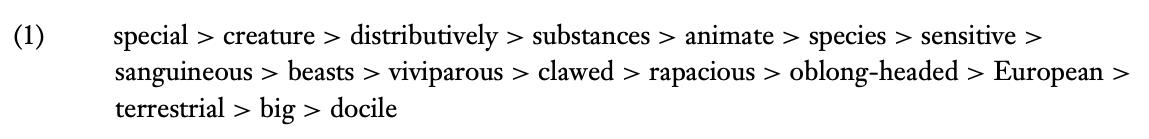
\includegraphics[width=1.0\textwidth]{WilsonsLanguageExample.png}
        \caption{Wilson's expression of "dog" \parencite{goodall2022article}}
        \label{fig:wilsonslanguageexample}
\end{figure}

% It is from this category that the constructed languages used in the present study come from.
% Speak more about details of these IALs here? Or in the data section?

In the 19\textsuperscript{th} and 20\textsuperscript{th} centuries the focus for language construction, especially in Europe, shifted to that of making international auxiliary languages (IALs) intended to better enable communication across language barriers, i.e., people who do not share a similar language \parencite{goodall2022article}. Notably, this means they were generally designed to resemble natural language, with choice exceptions being the simplification of certain linguistic features. The surge in need for IALs correlated with the increase in prevalence and accessibility regarding international travel and communication at the time. Such languages were also described as "neutral" \parencite{Large1985book}, in the sense that individual advantages amongst speakers and learners would, theoretically, not exist due to IALs being second languages to everyone \parencite{Gobbo2016article}. That being said, many of the most prominent examples (e.g., Volapük, Interlingua, Esperanto, Ido) are derived only from the Indo-European language family \parencite{Novikov2022article,goodall2022article}, so such a description might not be apt. 

% Discuss all of the IALs here? Or only some? Or is it unnecessary to discuss them in such detail anyways?
% [DELETED] clubs were soon founded and spread around Europe and then to the United States and China, too \parencite{okrent2009book}. At its peak nearly a decade later, there were over two hundred societies and clubs, three hundred learning manuals \parencite{Gobbo2016article}, and twenty-five routinely published Volapük journals \parencite{okrent2009book}.
% (Gobbo 2008) for discussing Ido

As the constructed languages examined and used in the dataset of the present work are all IALs, it would be beneficial to introduce them in more detail here. Volapük was made in 1879 by Catholic German priest Johann Martin Schleyer, who believed it was given to him by God. Argued to be the first successful constructed language due to amassing so many supporters \parencite{Gobbo2016article}, it soon died out in favor of Esperanto, which Ludwik Lejzer Zamenhof published in 1887.

% Mention other kinds of constructed languages, i.e. experimental or artistic ones like Solresol, Laadan, Lojban? (Adelman 2014)
Finally, 

While they all share the defining feature of having been purposefully created, their other features (e.g., phonetic, morphological, syntactical, lexical, orthographic) can vary immensely depending on factors such as, for example, their intended purpose for use or the other languages they draw from. An example of this was observed by \textcite{Gobbo2016article} in secret languages, specifically their tendency to have more complicated features, such as morphological irregularities, "in order to preserve their secrecy." Contrast to this are IALs, which have the opposite tendency for the sake of ease of communication and second-language acquisition, reflected in commonly assigned features such as SVO word orders, head-initial relative clauses, fronted \textit{wh-}phrases, and morphological regularity \parencite{goodall2022article,Gobbo2016article}. Section \ref{ssec:priorstudies} further examines research focused on linguistic features of these languages. 

In addition to classification based on their intended communicative functions, i.e. as philosophical or international auxiliary languages, there are also taxonomies based on other criterion. For example, another frequently used distinction is that of \textit{a priori} and \textit{a posteriori} \parencite{Schreyer2021article,Gobbo2008article,Schubert1989inbook,Schubert2001book,Novikov2022article,Adelman2014article,Tonkin2015article}. Languages described as being \textit{a priori} are structurally entirely new \parencite{Tonkin2015article} and not based on existing languages, whereas so-called \textit{a posteriori} languages are the opposite, drawing from aspects of specific natural languages \parencite{Schreyer2021article}. \textcite{Gobbo2008article} also proposed the dichotomy of \textit{exoteric} (secret) and \textit{esoteric} (public) languages, derived from \textcite{Bausani1974book}. Similar to critiques regarding the distinction between constructed and natural, such dichotomies for categorizing constructed languages are also argued by some linguists to be more accurately described as scales instead, with many languages falling somewhere in the middle \parencite{Novikov2022article}.

A two-dimensional classification schema for constructed languages containing several notables examples is shown in Figure \ref{fig:taxonomyplannedlanguages} \parencite{Gobbo2016article}.

% Include chart "taxonomy of planned languages" from Gobbo 2016 (fig 2). IMPORTANT QUESTION!!!!!! IS IT OKAY TO BORROW DIRECTLY LIKE THIS AS LONG AS I CITE IT?

\begin{figure}
  \centering
        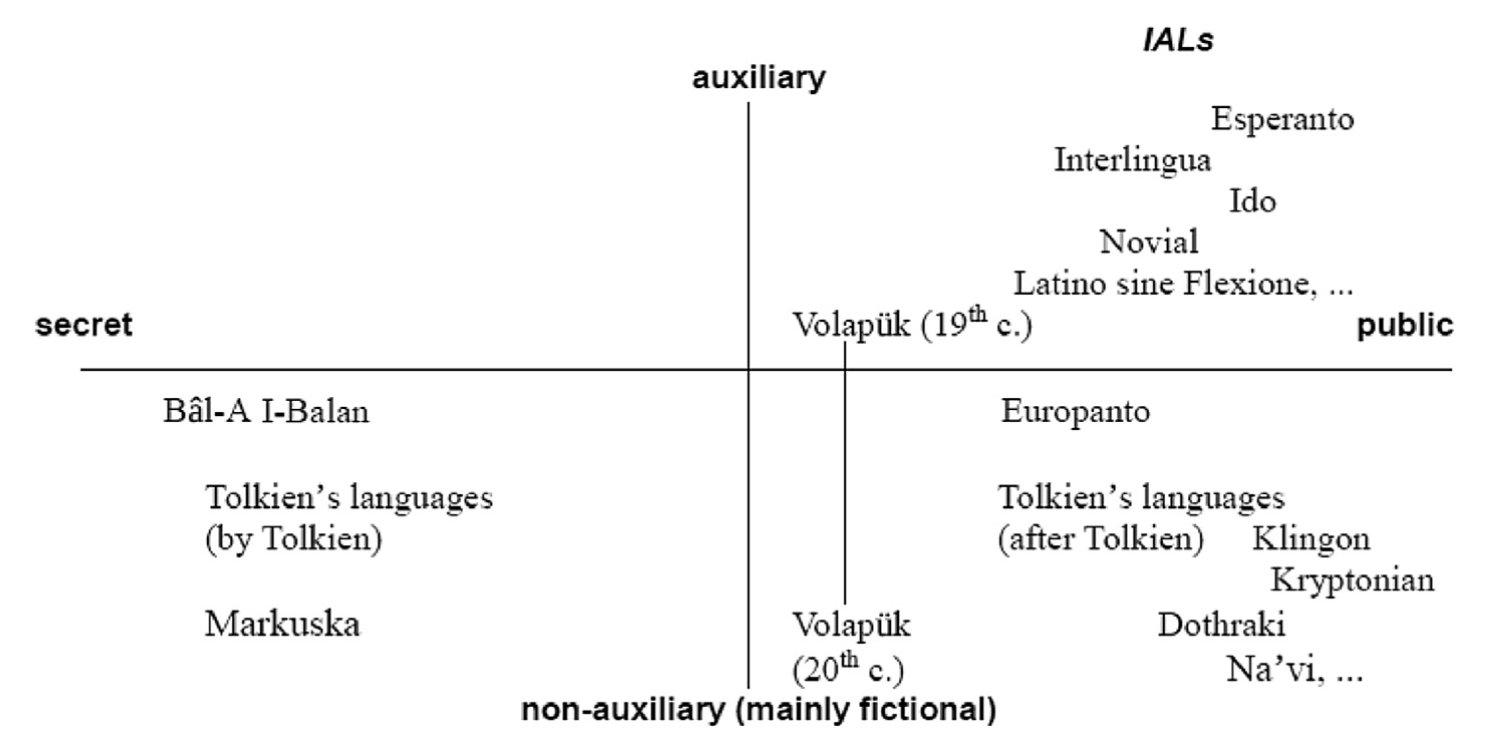
\includegraphics[width=1.0\textwidth]{TaxonomyOfPlannedLanguages.png}
        \caption{A taxonomy of constructed languages \parencite{Gobbo2016article}}
        \label{fig:taxonomyplannedlanguages}
\end{figure}

\subsection{Prior Studies}
\label{ssec:priorstudies}

% Prior studies comparing natural and constructed languages by linguistic features, prior studies on classification tasks for constructed languages

% Examining the Inductive Bias of Neural Language Models with Artificial Languages (White 2021)
% Are planned languages less complex than natural languages? (Gobbo 2016) 
% Constructed languages are processed by the same brain mechanisms as natural languages (Malik 2023)
% Constructive Linguistics for Computational Phraseology: the Esperanto Case (Gobbo 2019)
% On Pragmemes in Artificial Languages (Libert 2016)
% Authorship attribution, constructed languages, and the psycholinguistics of individual variation (Juola 2017)
% Sign language : a systematic review on classification and recognition (Sasidharan 2024)
% Morfessor-enriched features and multilingual training for canonical morphological segmentation (Rouhe 2022)
% Complexity measurement of natural and artificial languages (Febres 2014)
% Natural and Artificial International Languages: a Typosogist's Assessment (Comrie 1996)
% Evaluating the Irregularity of Natural Languages (Gomez 2017)
% The word entropy of natural languages (Bentz 2016)
% Entropy of natural languages: Theory and experiment (Levitin 1994)
% Morphology Matters: A Multilingual Language Modeling Analysis (Park 2021)
% Can Type-Token Ratio be Used to Show Morphological Complexity of Languages? (Kettunen 2014)
% What do complexity measures measure? Correlating and validating corpus-based measures of morphological complexity (Coltekin 2022)
% The effects of type and token frequency on word length: a cross-linguistic study (Berg 2022)
% Token-based typology and word order entropy: A study based on Universal Dependencies (Levshina 2019)
% Crosslinguistic Corpus Studies in Linguistic Typology (Schnell 2022)
% Data-driven Model Generalizability in Crosslinguistic Low-resource Morphological Segmentation (Liu 2022)
% The development of morphological complexity: A cross-linguistic study of L2 French and English (De Clercq 2016)
% Bentz's papers
% Multiple studies on artificial language acquisition
% Prior studies on entropies of languages
% Prior cross-linguistic studies examining linguistic features like TTR of constructed/natural languages
% (Gobbo 2016) "The literature on planned languages is abundant and diverse, written in many languages and quite often outside of the usual peer-review system (Blanke, 2003), but in comparison to natural languages there are only few specific studies addressing the complexity of planned languages from the point of view of learnability. For instance, Jansen (2012) addresses the problems of learning the reflexive pronouns in Esperanto. In his review of the doctoral dissertation of Heil (1999), who compares the grammar reduction in French-based creoles and planned languages, Haitao (2001) rightly points out that more comparative work in this field is needed, and on a more solid basis."

In contrast to the abundance in literature and cross-linguistic analyses done on natural languages, similar research which also includes constructed languages is relatively sparse. In particular, while there is research that analyzes specific instances of linguistic differences between certain natural and constructed languages, large-scale cross-linguistic studies which utilize computational methods to classify the two based on linguistic features are practically nonexistent. Consequently, the present study is a somewhat novel approach. However, there is precedent for this research and the specific features examined, as well as computational approaches used, which this section will describe.

As previously mentioned, the creation of IALs such as Esperanto often involved the intentional simplification of particular language features to facilitate language acquisition, for instance having more regularity in their morphological systems. Intuitively, then, one would assume this translates to measurable differences in various aspects of linguistic complexity when compared to natural languages, which often have irregularities as a result of their development and evolution. 

\subsection{Computational Methods}
\label{ssec:computationalmethods}

\newpage
\section{Methodology}
\label{sec:methodology}

In this section, I explain in greater detail the dataset, APIs, and libraries used, as well as the approaches and steps taken to arrive at my results. Because of the broad nature of this study, several different experiments are done to test various linguistic features. Namely, these features are measurements of morphological complexity, type-token ratio (TTR), moving-average type-token ratio (MATTR), lexical entropy, text entropy, and character and word distribution entropies. Once these were calculated for each language, the task became that of binary classification using these values with the use of two models: a one-class support vector machine (SVM) and a decision tree. 

\subsection{Data}
\label{ssec:data}

In total, twenty-four languages are analyzed in this study. Six of these are constructed languages: Esperanto, Interlingua, Lingua Franca Nova, Volapük, Kotava, and Ido. The remaining eighteen are natural languages: German, English, Spanish, Polish, Vietnamese, Indonesian, Turkish, Tagalog, Hungarian, French, Finnish, Italian, Dutch, Occitan, Danish, Swedish, Afrikaans, and Icelandic. 

% For conlangs, how should I call the languages they are drawn from? "Language influences" or is there a better way to say it?

\begin{table}[h!]
\centering
\renewcommand{\arraystretch}{1.5}
\begin{tabular} {|p{3cm}|p{3cm}|p{3cm}|}
\hline
\textbf{Language} & \textbf{Language Influences} & \textbf{Word Order} \\
\hline
Esperanto & & SVO \\
Interlingua & & \\
Lingua Franca Nova & & \\
Volapük & & SVO \\
Kotava & & \\
Ido & & \\
\hline
\end{tabular}
\caption{}
\label{tbl:conlangs}
\end{table}

% Plot the languages + their language families to have some kind of visual comparison (table also works, include some data points for comparing each language i.e. number of speakers, word order (what do I do when it isn't clear due to having a more free word order, like for Esperanto, Finnish, etc?))
% Explain why I had to build my own corpus rather than using one that already exists. What limits are present as a result of having to build my own? 
% Discuss their language families, writing scripts (why not Japanese or Chinese?), and why those 4 constructed languages specifically
% Explain which natural language families the conlangs are based on, and surface level distinctions they may have
% von Oostendorp's Constructed Language and Linguistic Theory cites information about Ido (and Interlingua) around pages 7-8, how it is different from Esperanto
% Write more in-depth about Ido, Esperanto, Interlingua, Volapük, and Lingua Franca Nova. Who created them, how many estimated speakers, their purpose for being created, etc. etc.
% Write differences between Ido and Esperanto, using specific examples (for ex, from Goodall 2022), same for Interlingua. For example, a chart comparing words/grammar in all the languages, like on page 6.
% Mention how for some calculations done in this work, such as entropy, domain and corpus size are important and can cause results to vary
% Comrie 1996 also breaks down Esperanto with examples
% Lindsedt 2006 writes about considering Esperanto as a natural language and breaks down properties of it as well. Gobbo 2011 (section 4) breaks down further the specific languages Esperanto comes from
% Write about the Eurocentricism of the constructed languages used here (their inspirations/influences) and how that may affect the results
% Mention the drawbacks of relying on Wikipedia data, such as difference in authors, etc
% Why didn't include lojban? or Novial? (Available data for it is way smaller)

To briefly introduce the constructed languages used here, Esperanto is the most widely spoken constructed language

% "and more niche" with how many speakers?
% Discuss LFN being inspired by Mediterranean Lingua Franca https://en.wikipedia.org/wiki/Mediterranean_Lingua_Franca

The final constructed language used in this study is Lingua Franca Nova, created by Dr. C. George Boeree. Compared to the others discussed so far, it is much more recent in its creation, having first appeared in 1998 online. As a result of being both newer and more niche, there is considerably less existing research related to it. Its inclusion in my dataset is primarily due to it being used on Wikipedia as an available source language, and thus also having a Wikimedia dump file.

As this study is cross-linguistic in nature, it would naturally be ideal to use parallel text corpora, as this would enable more conclusive comparative and comprehensive analysis. However, finding already existing parallel corpora that also includes constructed languages, particularly less common ones, posed a bit of a challenge. 

% Include Blanke's (Schubert2001book) description of Esperanto as the only successful planned language

% Example link to one of the files used: https://dumps.wikimedia.org/novwiki/20240701/ then select novwiki-20240701-pages-articles-multistream.xml.bz2 1.4 MB
% Which languages' files did you limit (using the max_articles variable) with the script? The biggest files (eo, da, fi, tr, id, vi, hu, sv, nl, pl, it, es, fr, de, en) I gradually limited the max number of files to be extracted from the dumps; max 50000 for eo, 

The corpora were compiled using Wikimedia database dumps---large files containing Wikipedia articles for a given language which are formatted in XML. The corpus sizes were constricted to be comparable in length in number of words, while still maintaining complete sentences. In terms of file size, the smallest dump was Lingua Franca Nova, so its was the minimum value used to shorten the others. 

% Previously (in 2023) used a min value of 650000 words, now (in 2024) using min value of 630000 words
% Genre/domain of texts? Do all dumps have the exact same articles? How does this affect the experiment and results?
% Not gold standard corpus, its quality depends on many different variables (i.e. the wikipedia contributors who wrote the articles)
% Give a breakdown of the corpora data, for example the number of words/sentences for each language

\subsection{Data Preprocessing}
\label{ssec:datapreprocessing}

Preprocessing text data is essential for NLP tasks. As this study covers a broad range of different languages and includes constructed languages, which often have less resources available, meticulous effort was made to obtain as close to a parallel set of corpora as possible and to clean the text thoroughly. 

% Preprocessed by excluding characters not in a language's alphabet, to attempt to account for words in foreign languages being used in the text data, however this has drawbacks in that it also excludes loanwords or proper nouns at times too. Additionally, I removed only the individual characters themselves, is it better (or possible?) to remove the entire word that they are part of instead? Or does it not make a difference? For example, in Kotava there is no letter 'h', the proper noun 'hiroshima' therefore would become 'irosima' with my method. 
% Wanted to keep full sentences (why?), so there is not exact same word counts/sentence counts for all files. Include chart of total words/sentences for each language file?
% Mention why the WikiExtractor script was used in the first place
% Ex: python WikiExtractor.py --infn ~/Downloads/enwiki-20240701-pages-articles-multistream.xml.bz2
% Show some examples of the regex used from your code
% Show examples of before and after the preprocessing + show an example of the final preprocessed data

After extracting the text from the dump files through the use of WikiExtractor, a Python script \parencite{Attardi2015wikiextractor}, regular expressions were used to remove page titles, links, headers, fragments, and other extraneous symbols. The text was then made all lowercase and split by the periods---while also attempting to account for abbreviations---to make separate sentences, and all characters that were not part of the language's writing system were removed in an attempt to have only that language's words, without any foreign words that occasionally appear in the scraped Wikipedia texts. Remaining punctuation and numbers were also removed. The end result was a single corpus file corresponding to each language, with each line of the files being a single sentence. 

\subsection{Libraries and APIs}
\label{ssec:librariesandapis}

\subsubsection{Keras}
\label{ssec:keras}

\subsubsection{PyTorch}
\label{ssec:pytorch}

\subsubsection{NumPy, Pandas, and Matplotlib}
\label{ssec:numpypandasmat}

\subsubsection{scikit-learn}
\label{ssec:scikitlearn}

\subsection{Feature Extraction}
\label{ssec:featureextraction}

% Briefly explain what feature extraction is and why I use it in this study (?)
% Come back to edit later:
% Once the data had been preprocessed, some initial values were calculated to be used as a starting point for our investigation in comparing natural and constructed languages. These were Zipf's law of abbreviation, type-token ratio (TTR), moving-average type-token ratio (MATTR), and character and word distribution entropies.

% Mention in each subsubsection why the particular feature was extracted, why it was seen as a possible indicator or useful information in this experiment
% IMPORTANT: RUN EVERYTHING AGAIN. ONLY PRE-PROCESSING WAS FINISHED, 2 NEW LANGUAGES ADDED TO STUDY

\subsubsection{TTR \& MATTR}
\label{ssec:ttrandmattr}

TTR is a way of measuring lexical diversity. It is calculated using the following formula: \[TTR = \frac{\sum_{i=1}^{n}\delta(w_i)}{n}\]

A glaring issue with TTR, however, is that it can vary widely based on a text's length. The longer a particular text, the higher the likelihood of repetition occurring. There have been several solutions proposed to address this issue, one being MATTR. MATTR is given in the formula \[MATTR_i = \frac{TTR_1+TTR_2+...+TTR_i}{i}\]

\subsubsection{Morphological Complexity}
\label{ssec:morphologicalcomplexity}

% Mention the root languages the conlangs are based on (i.e. Esperanto and German) to explain/describe some of the morphological complexity of said conlang
% "A popular algorithmic way to approximate the morphological complexity of a language has been Patrick Juola’s (1998, 2008) suggestion of distorting word structures by using a unique random number for each different word type. After distortion, the data is compressed using a compression algorithm. Then the size of the compressed original word file is divided by the size of the compressed distorted word data file. The result tells the complexity of each language’s morphology on the basis of Kolmogorov complexity that the compression algorithm approximates." (Kettunen 2014)

The morphological systems of each language were analyzed using Morfessor, 

\subsubsection{Zipfian Distribution}

% Zipfian distribution of natural languages vs constructed languages, refer to Bentz 2023
% Zipf’s word frequency law in natural language: A critical review and future directions (Piantadosi 2014)

\subsubsection{Entropy}
\label{ssec:entropy}

In information science, entropy means... 
In linguistics, entropy refers to...
Surprisal...

% Calculated character, word, text, and lexical entropies

The entropy was calculated for the character and word distributions in each of the corpora, given by the following formula: \[H = -\sum_{i=1}^{n}p_{i}\log_{2}p_{i}\]

\subsubsection{Perplexity}
\label{ssec:perplexity}

Perplexity is related to entropy...
Cross-entropy as the loss function...

\subsubsection{PCA}
\label{ssec:pca}

% "To analyze whether measures include multiple dimensions or not, we perform dimensionality reduction using principal component analysis (PCA). The intuition here is that if the measures differ in what they measure, the explained variance should be shared among multiple principal components. Furthermore, if the lower-order principal components measure meaningful dimensions of morphological complexity, we expect them to indicate linguistically relevant differences between languages." (Coltekin 2022)

Principal Component Analysis was performed for dimensionality reduction. 

% Discuss variance ratio

\begin{figure}
  \centering
        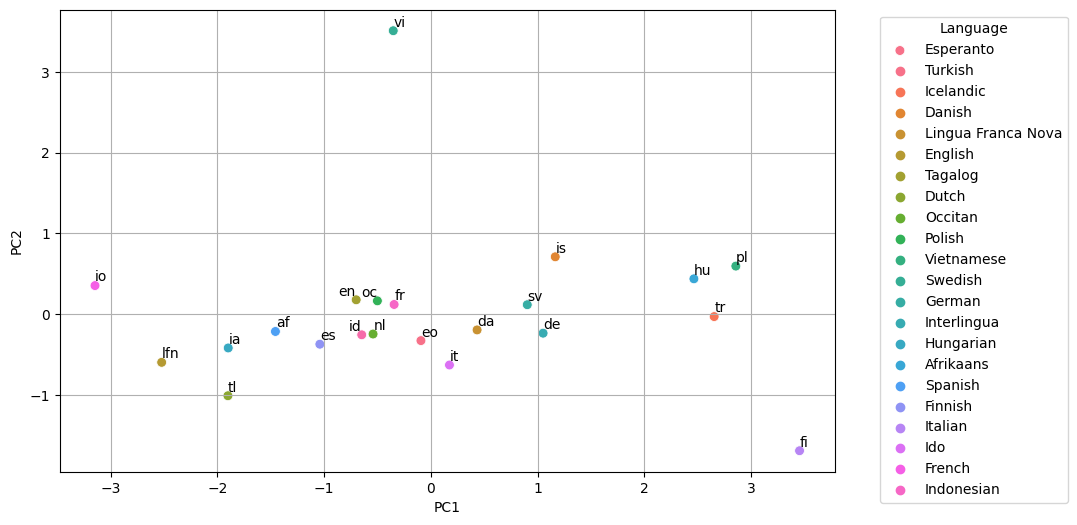
\includegraphics[width=1.0\textwidth]{pcaanalysis.png}
        \caption{Principal Component Analysis on TTR, MATTR, Word and Char Distribution Entropy}
        \label{fig:pcaanalysis}
\end{figure}

A script was used to increase readability of the text in the graph\footnote{https://github.com/Phlya/adjustText}.

\subsection{Classification Models}
\label{ssec:classification}

% Visualizing the features (in a graph) prior to classification to analyze whether a linear or nonlinear model is required and why 

\subsubsection{Decision Tree}
\label{ssec:decisiontree}

Decision Tree Classifier...

\begin{figure}
  \centering
        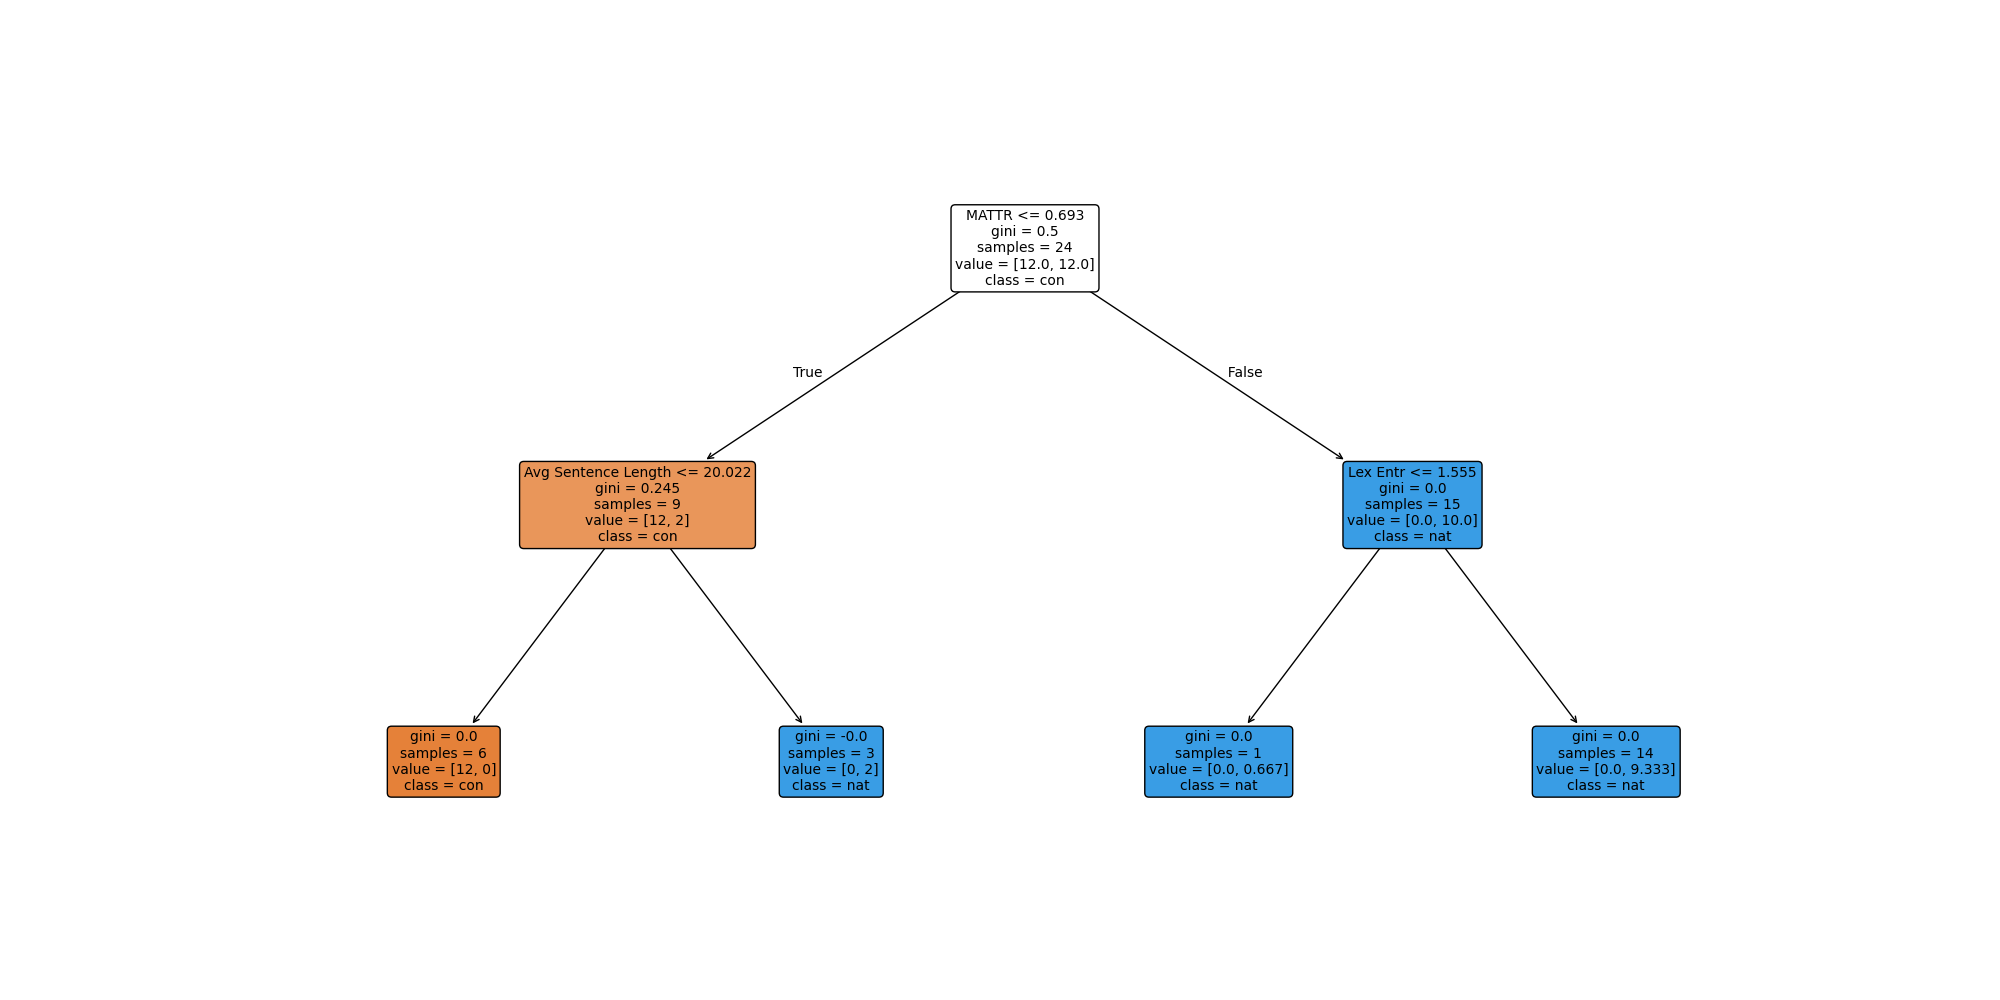
\includegraphics[width=1.0\textwidth]{decisiontree.png}
        \caption{Decision Tree Classifier}
        \label{fig:decisiontree}
\end{figure}

\subsubsection{Outlier Detection}
\label{ssec:outlierdetection}

\newpage
\section{Results}
\label{sec:results}

\newpage
\section{Discussion}
\label{sec:discussion}

% Mention expectations (e.g. the conlangs coming from European languages, so the models might confuse these with the natural languages when classifying the two) and how they compare to the results
% Come back to the question/topic of linguistic universals, how do these results fit into the debate?

\newpage
\section{Conclusion}
\label{sec:conclusion}

\subsection{Future Work}
\label{ssec:futurework}

The research presented in this thesis is far from encompassing all there is to the topic of defining language, and distinguishing between constructed and natural language. At present, this is an area of research with ample room for potential development. 

Limiting factors: number of languages and which languages/language families, lack of real parallel corpora, problems associated with low-resource languages, relatively narrow scope of experimentation,

\newpage
\section{Acknowledgments}
\label{sec:acknowledgments}
I would like to thank ....

\newpage
\printbibliography

\newpage
\section{Appendices}
\label{sec:appendices}

Here I...

\begin{table}[h!]
  \centering
  \renewcommand{\arraystretch}{1.5}
  \begin{tabular} {|p{3cm}|p{3cm}|p{3.5cm}|}
  \hline
  \textbf{Language} & \textbf{Number of Words} & \textbf{Number of sentences} \\
  \hline
  Icelandic & 629995 & 41847 \\
  German & 629987 & 37261 \\
  Polish & 629997 & 42138 \\
  Ido & 629990 & 43496 \\
  Afrikaans & 629994 & 30737 \\
  Kotava & 617400 & 48145 \\
  Hungarian & 629946 & 39916 \\
  Lingua Franca Nova & 628683 & 32188 \\
  Danish & 629999 & 38260 \\
  Spanish & 629978 & 24886 \\
  Interlingua & 629996 & 32229 \\
  French & 629983 & 27248 \\
  Occitan & 629998 & 33762 \\
  Esperanto & 629994 & 33317 \\
  Dutch & 629997 & 34627 \\
  Turkish & 629995 & 43573 \\
  English & 629958 & 29574 \\
  Tagalog & 629989 & 29855 \\
  Swedish & 629998 & 36370 \\
  Vietnamese & 629958 & 21115 \\
  Italian & 629987 & 24487 \\
  Volapük & 629999 & 55920 \\
  Indonesian & 629997 & 34683 \\
  Finnish & 629994 & 52637 \\
  \hline
  \end{tabular}
\caption{Lengths of each text after pre-processing.}
\label{tbl:preprocessedtexts}
\end{table}

\end{document}

